\documentclass[11pt]{article}

\usepackage[margin=1in]{geometry}
\usepackage{setspace}
\usepackage{enumitem}
\usepackage[hidelinks]{hyperref}
\usepackage{titlesec}
\usepackage{pdfpages}

\setstretch{1.08}
\setlength{\parindent}{0.25in}
\setlength{\parskip}{0.4em}
\setlist[itemize]{leftmargin=1.4em,itemsep=0.2em,topsep=0.25em}
\titleformat{\section}{\large\bfseries}{\thesection}{0.5em}{}
\titlespacing*{\section}{0pt}{0.9em}{0.4em}

\begin{document}

\begin{center}
{\Large \textbf{Writing Lab Reflection --- Session 2}}\\[0.35em]
EDCI 59100-016: Literature Review\\
Md Kamruzzaman Kamrul\\
Summer 2026
\end{center}

\vspace{0.5em}

\section*{Coach Report Record}

\noindent\textbf{Report source:} Purdue OWL Report email (noreply@mywconline.com), received June 18, 2026 at 5:15 PM\\
\textbf{To:} Md Kamruzzaman Kamrul \textless mkamrul@purdue.edu\textgreater\\
\textbf{Client:} MD KAMRUZZAMAN KAMRUL\\
\textbf{Staff or Resource:} Katie G.\\
\textbf{Appointment date:} June 18, 2026, 4:00 PM -- 5:00 PM (Online session)\\
\textbf{Document type:} Scholarly Article\\
\textbf{Session focus:} Logical sequences/organization; Content development/support of main ideas

\medskip

\noindent Katie's report reads in full:

\begin{quote}
Hi Kamrul,

It was nice to get to talk to you today! I'm glad I got to hear more about your project directly from you!

Today we talked about some of your concerns about structure. You shared the PRISMA standards for scoping analysis, and we talked about using those as a checklist to make sure that you have everything you need to in this paper.

You were not sure about whether or not to keep your descriptive analysis in section 3, since it is not required by the PRISMA standards. My biggest advice for that is to think about whether or not the descriptive analysis is helpful to your reader. Do they need it? Does it add a lot of important information to your literature review? If not, I think you can cut it. If there are a couple of sections that are helpful or important, you can always include those and cut the rest.

We also talked about how you wanted to propose a framework in your literature review. For this, I think you should look at other literature reviews in this journal. Do they also propose a framework? If so, how do they do it? You can then take these lessons and decide how you want to propose your own framework. You mentioned that you found the framework important because it is part of identifying the research gap when it comes to using VLMs for construction management.

I hope this was helpful, and feel free to come back to the OWL if you want to talk more about this or any other writing!

Best,

Katie
\end{quote}

\section*{Reflection}

Working with Katie G. was a productive and focused session. She asked to read the PRISMA-ScR standards alongside the draft manuscript, which grounded the entire discussion in concrete structural decisions rather than general writing advice. This made the hour efficient and immediately useful. The session addressed two specific uncertainties I had held since completing the draft: whether to retain the full descriptive analysis chapter and how to position the Three-Layered Spatiotemporal VLM Framework within the paper.

On the first point, Katie clarified that PRISMA-ScR does not mandate a stand-alone descriptive analysis chapter. Her advice was to evaluate each subsection individually by asking whether it adds information the reader genuinely needs to follow the thematic analysis. Applying that test, I plan to retain the publication trend figure (Figure 1) and the master charting table (Table 7), because they directly establish the empirical foundation for the paradigm-by-paradigm analysis in Section 4. The publication trend figure shows the post-2022 acceleration that explains why VLMs displaced unimodal CV as the dominant approach, and the charting table provides the auditable evidence base from which all thematic claims are drawn. I plan to condense or remove the journal landscape breakdown (Table 3), the automation level table (Table 4), and the evaluation metrics section (Table 6), because those findings are already addressed analytically in the Discussion. Streamlining these sections will reduce the chapter's ``data dump'' feel and tighten the connection between Section 3 and Section 4.

On the second point, Katie suggested I examine how other scoping reviews published in \textit{Automation in Construction} handle framework proposals, so that my own approach is consistent with the journal's conventions. I will search recent AiC scoping reviews to determine whether frameworks typically appear as contributions introduced in the Introduction or as analytical tools presented at the start of the thematic analysis. If other AiC papers introduce their frameworks early to orient the reader, I will move the Three-Layered Framework description to the Introduction and reference it throughout Sections 4 and 5. If frameworks are more commonly introduced in the analysis chapter, the current positioning in Section 4.1 is appropriate. Either way, I will make the framework's role explicit: it is both an analytical scaffold for organizing the 56 included studies and a contribution to identifying the research gap, since no prior review has classified VLM applications in construction according to an architectural paradigm model.

\clearpage
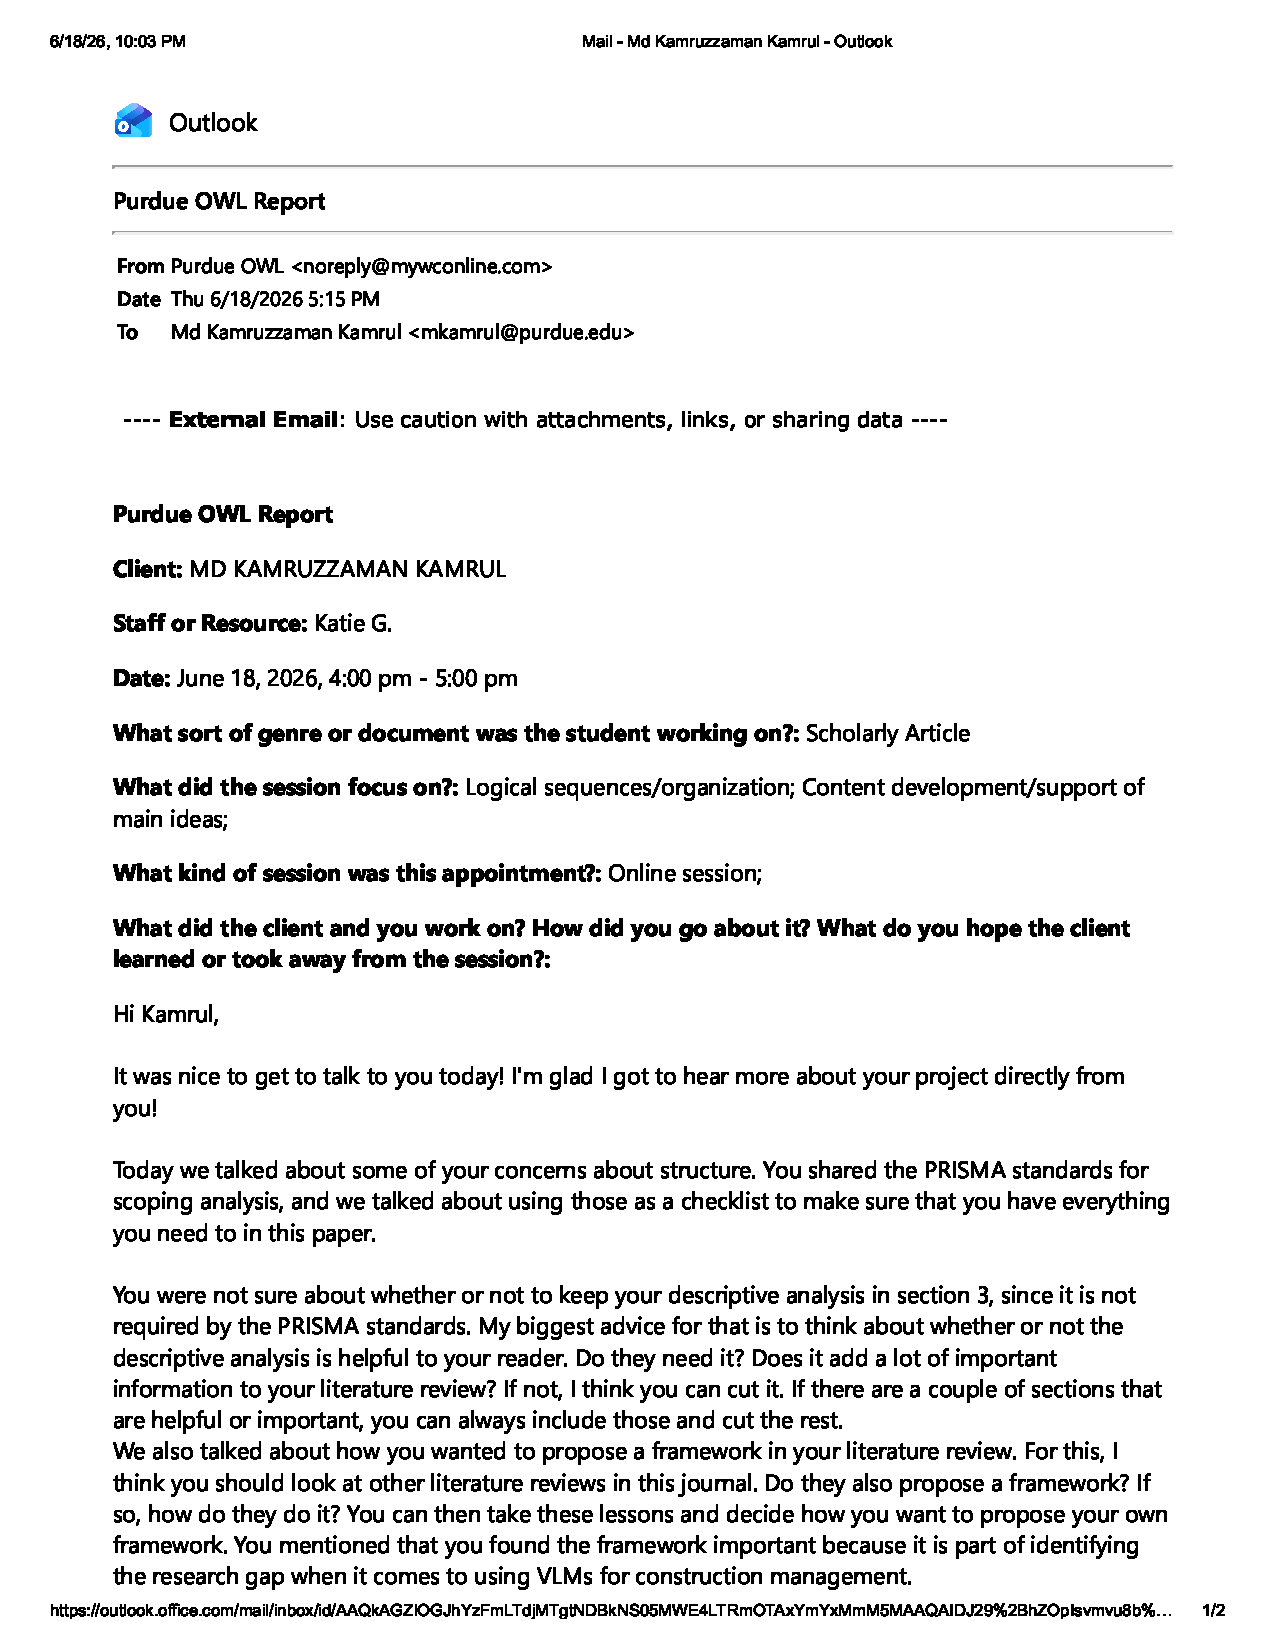
\includepdf[
  pages=-,
  pagecommand={\thispagestyle{plain}},
  scale=0.92
]{OWL_Coach_Report_KatieG_June18_2026.pdf}

\end{document}
